% !TEX root = Skin_Lesion_Classification_Using_Machine_Learning.tex

\section{Skin Lesion Classification Using Convolutional Neural Networks [SE]}\label{sec:cnn}
For the second part of this project, we used convolutional neural networks (CNNs) to classify the images containing skin lesions. 
We apply transfer learning to pretrained networks on the ImageNet dataset. All training and testing was done on a Nvidia Tesla P100 with 16GB of video memory via Google Colab. The model and its input pipeline was developed using Tensorflow and evaluated using the same Sklearn functions as in section \ref{sec:svm}. 
\subsection{Architecture [SE]}
We use the EfficientNet models for our prediction pipeline.
The base model B0 uses the standart ImageNet input size of $224 \times 224$, the models B1 to B7 scale that base architecture and allow much larger input sizes. The models are scaled uniformly in resolution, width and depth. This helps them to achieve state of the art performance on standart datasets while being smaller and faster then conventional architectures \cite{tan2019efficientnet}.

In our work, we manly use the models B3 and B4 which have an input size of $300 \times 300$ and $380 \times 380$ respectively. 
Those models outperformed resnet and densenet architectures in initial testing by a large margin. While the step from model B2 to B3 brought a significant performance improvement, the results of B3 and B4 were relatively similar. Larger models could not be trained enough epochs because of resource constraints.

For our final model, we only add global average pooling and one dense classification layer with softmax activation to the pretrained network. We tried adding additional fully connected layers in between so that the number of neurons don't decrease so fast (1536 to 8 for B3) but this did not bring an improvement. 

\subsection{Data Augmentation and Input Strategies [SE]}\label{sub:cnn_input}
We used the tensorflow.data API to handle the large dataset efficiently. The batches of training data are automatically loaded in the background only when they are needed. 
To increase the variety of the dataset, we applied online data augmentation. These included randomly flipping and rotating images, as well as random changes in contrast brightness and hue. The larger images are then resized so that they fit the original size of the images from the HAM10000 dataset. The aspect ratio is kept at this operation. 
The input for the network consists of random crops of same size of these augmented images. 

A different strategy without augmentation is applied to the validation and test data. We use equally spaced crops as seen in the last years challenge \cite{gessert2018skin}.
Each image is divided into six by six overlapping cops. All crops share the size of of the training data. 

\subsection{Learning and Testing [SE]}
The training is done using the Adam optimizer. We apply a learning rate schedule to reduce the learning rate every 20 epochs. This helped the loss to decrease continuously during training procedure. 

The imbalanced dataset is handled as before by class weights. Every sample gets a weight assigned inversely proportional to its frequency in the dataset. The strategie proofed to be much more efficient in our tests than oversampling the less frequent classes. 
A batch size of 32 is used when ever possible and reduced for larger models to fit our GPU memory. 
In the first stage, we only train our final classification layer for 50 epochs. After that, the lower convolutional layer of the base model are unfrozen and also fitted to our dataset. This fine tuning of the more specialized convolution kernels gave us a big performance improvement. We train these layers using a low learning rate in several stages for an additional 75 epochs.  % #TODO more precise? 
Our final model was an ensemble of the B3 and B4 model. The predictions of both networks were averaged a the end. That technic improved the accuracy by tree percent points. The final model was able to archive a validation accuracy of 85.31\%. 

\subsection{Consideration of Meta Data [HBT]}

The Neural Networks with multiple inputs when the network require data from multiple sources or in different formats. For example, networks that require image data captured from multiple sensors at different resolutions. In many researches, the use of different type of data along with the image data for classification in deep learning has shown the considerable improvement in image classification\cite{love},\cite{melan}. The metadata is merged within the same pixel matrix of the image in each RGB layer which enriches the extraction of features, has shown significant improvement in accuracy in this research\cite{melan}. The image metadata is used nonparametrically to generate neighbourhoods of related images using Jaccard similarities, then used a deep neural network to blend visual information from the image and its neighbours in this research \cite{love}. McAuley and Leskovec pioneered the study of multilabel image annotation using metadata, and demonstrated impressive results using only metadata. In hope of improvement of accuracy mixed data approach is used.

% #TODO I'm sorry but that (above) aren't complete english sentences. I only partly get what you want to say

Including the metadata into the neural netwok is challenging. In contrast to the SVM based approach, the metadata is here in a different format then the image data. For that reason we created two separate networks and merged them. One branch is a Multi-Layer Perceptron (MLP) model that is designed to handle metadata and a second branch is a cnn for image data. Finally, these two branches are concatenated to have a final model for training.

The sex and position information of the metadat is converted to one-hot numpy arrays, the age is used as an numerical value. The MLP model consists of 4 layers with relu activation function with (128,64,32,8) neurons respectively. It has two inputs, age and sex. 
The conventional customized CNN model with 3 layers, with 3x3 filter size and (16,32,64) depth respectively and stride of 2 is chosen. Padding is done to the images to maintain the same length. Another CNN model with EfficientNet B4 for transfer learning followed by GlobalMaxPooling and 2 Dense layers with (512,8) neurons with SoftMax activation to the pretrained network. The transfer learning is performed using both the EfficientNet model and conventional CNN for better approximation of expected outputs. The cnn is trained the same way as before. 

\begin{figure}[h]
    \centering
    % include first image
    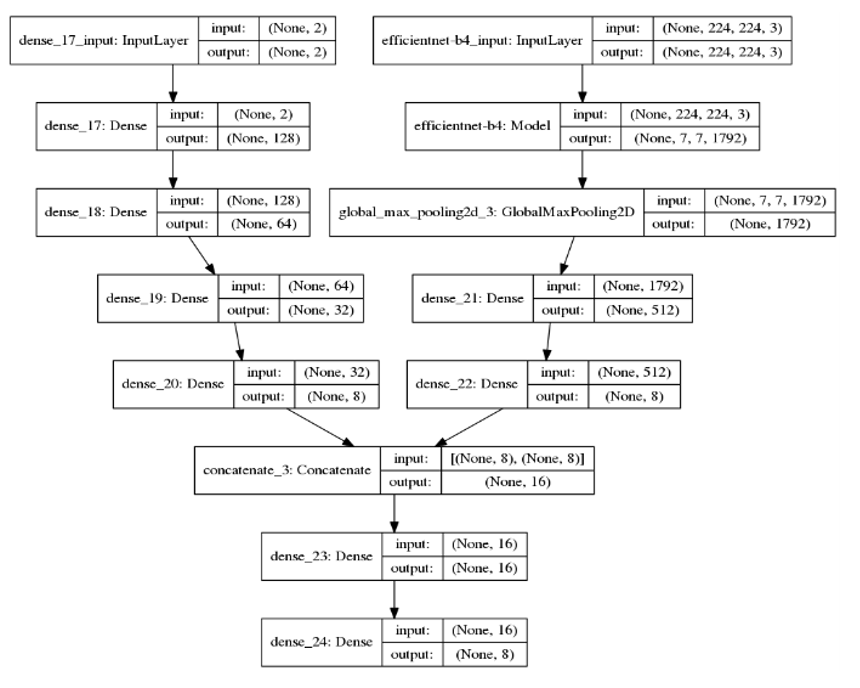
\includegraphics[width=.75\linewidth]{pictures/model.PNG}  
    \caption{Multi \- Input model that includes both CNN and MLP branches to handle mixed data.}
    \label{fig:model}
\end{figure}
% #TODO this picture is way to small to read

Figure \ref{fig:model} shows the Multi-Input model which combines both networks. 

Due to technical problems concerning the connection of tensorflow and keras, we could not use the image input pipeline described in section \ref{sub:cnn_input}. 
A validation accuracy of 53.63\% was achieved using the Multi-Input model. There is huge requirement of improvement in image data pre-processing techniques, hyper-parameter tuning, extracting features from image related to metadata for multi-input model as compared CNN model by considering only image data. Since the images are loaded using Open CV at onetime without using any Data Loading Pipeline, the training was taking very long time for each epoch. Normalizing is done at once for a whole image array is not efficient way and proved by experimenting it.
The accuracy is better for CNN model with a pre-trained EfficientNet model. Since the computational problems caused by OpenCV library in high resolution image data loading as input to multi-input model requires implementation of precise image processing techniques and a precise regularization with the loss obtained from model. The learning has to be regulated by considering metadata with respect to image data. Image augmentation and few other techniques may enhance the accuracy.  
